
\subsection*{task 2.4 [20 points] \\[1ex] solving the Oja flow}

In the \texttt{Data} folder for this exercise, you will find the file
\begin{quote}
    \texttt{GaussianSample3D.csv}
\end{quote}
which contains a (zero mean) data matrix $\mat{X} \in \mathbb{R}^{3 \times 250}$ whose columns $\vec{x}_i$ represent 3D data points. To read this matrix into memory and check its size, you may use
\begin{python}
X = np.loadtxt('GaussianSample3D.csv', delimiter=', ')
m, n = X.shape
print (m, n)
\end{python}

Given this data matrix, compute the sample covariance matrix
\begin{align*}
\mat{C} & = \frac{1}{n} \mat{X} \trn{\mat{X}}
\intertext{and its spectral decomposition}
\mat{C} & = \mat{U} \mat{\Lambda} \trn{\mat{U}}
\end{align*} 
and print the leading eigenvector, i.e. the eigenvector $\vec{u}_1$ belonging to the largest eigenvalues $\lambda_1$.

\begin{python}
# build the sample covariance matrix
C = 1/X.shape[1] * (X @ X.T)
# compute the spectral decompostion of the covariance matrix
# remember from the last assignment sheet that la.eigh is a
# good choice here, since the covariance matrix is symmetric
# V_eig: eigenvalues of C in ascending order
# U_eig: eigenvectors of C
V_eig, U_eig = la.eigh(C)
# show the eigenvector corresponding to the largest eigenvalue
# recall the ascending order of the eigenvalues
print("u_1:", U_eig[:, -1])
\end{python}

Now recall that, in the lecture, we studied the Oja flow, i.e. the following dynamical system
\begin{equation}
\label{eq:flow}
\dot{\vec{w}} = \bigl( \mat{I} - \vec{w} \trn{\vec{w}} \bigr) \mat{C} \vec{w}
\end{equation} 
where we simply write $\dot{\vec{w}}$ and $\vec{w}$ instead $\dot{\vec{w}}(t)$ and $\vec{w}(t)$. In other words, \eqref{eq:flow} is an ordinary differential equation w.r.t.~time $t$. 

We claimed that, for initial conditions $\vec{w}(0) = \vec{w}_0$ such that $\lVert \vec{w}_0 \rVert =1$, this flow will converge to the leading eigenvector of $\mat{C}$.

In this task, you are supposed to verify this using numerical methods (rather than mathematical proof). In other words, first initialize some unit vector $\vec{w}_0$ and then use Scipy's \keyword{odeint} method in order to numerically solve the differential equation in \eqref{eq:flow}.

The method \keyword{odeint} is contained in the module \keyword{scipy.integrate} and fairly well documented on the Web. Try to figure out for yourself how to use it. That is, see for yourself what kind of inputs it requires and what kind of outputs it yields.

\begin{python}
from scipy.integrate import odeint
# implement the differential equation
w_prime = lambda w, t: (np.eye(3) - w[:, None] @ w[None, :]) @ C @ w
# create a random unit vector as an initial guess
w_0 = np.random.uniform(-1, 1, size=(3,))
w_0 /= la.norm(w_0)
# solve the differential equation using scipy's odeint method
t = np.linspace(0, 3, 50)
w = odeint(w_prime, w_0, t)
# print approximation of u_1
print("w_t:", w[-1, :])
\end{python}

Once you have solved \eqref{eq:flow} for appropriate initial conditions, plot your result. In principle your plot should look something like this (not necessarily as fancy though):
\begin{center}
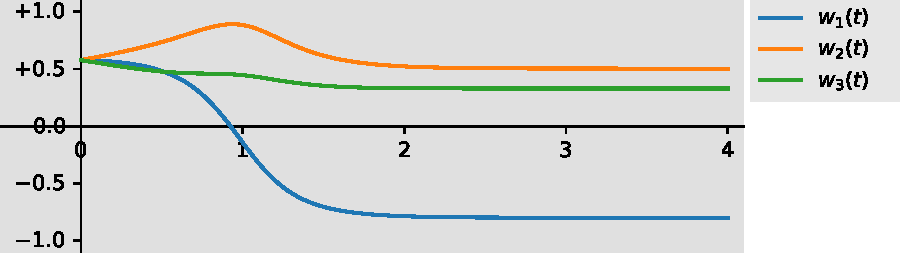
\includegraphics[width=\textwidth]{OjaFlow.pdf} 
\end{center}
\textbf{NOTE:} This result was obtained using $\vec{w}_0 = \frac{1}{\sqrt{3}} \vec{1}$. When you enter your result below, please use some random vector $\vec{w}_0$ with $\lVert \vec{w}_0 \rVert = 1$.
%%%%%
%%%%%
%%%%% enter your plot here, i.e. replace "placeholder.pdf" by the names of the graphics file you created
%%%%%
%%%%%
\begin{center}
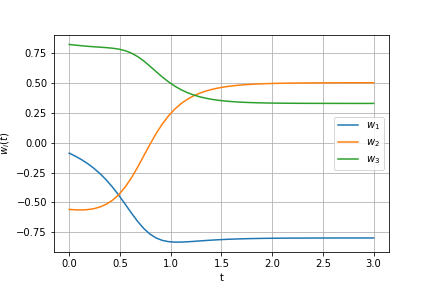
\includegraphics[width=0.7\textwidth]{Ex_02/Figures/OjaFlow.png} 
\end{center}
%%%%%
%%%%%
%%%%%
%%%%%
%%%%%

Compare the stable point the flow converges to to the leading eigenvector $\vec{u}_1$ you computed above. What do you observe? Also, experiment with different initial conditions / starting point for the flow. What do you observe?
\color{blue} \\[1ex]
%%%%%
%%%%%
%%%%% enter your discussion here
%%%%%
%%%%%
The two code fragments output the following:

$u_1$: [ 0.7988784 , -0.50319912, -0.32952077] \\
$w_t$: [ 0.79885363, -0.50324345, -0.32951316]

So one can see that $w_t$ is in fact an approximation of the leading eigenvector $u_1$ of the sample covariance matrix $C$. Depending on the initial condition for the flow it might happen that the the two vectors are of different sign, i.e. $w_t \approx -u_1$. This is represented by the cosine similarity converging to -1 instead of +1. However $-u_1$ is still a leading eigenvector of $C$.

\begin{figure}[h]
    \centering
    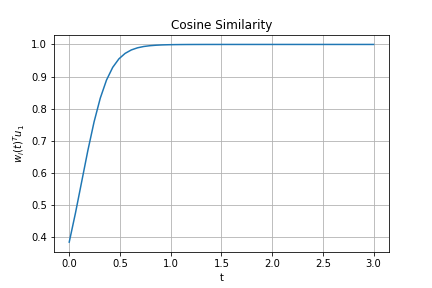
\includegraphics[width=0.45\textwidth]{Ex_02/Figures/CosSimilarity_positive.png}
    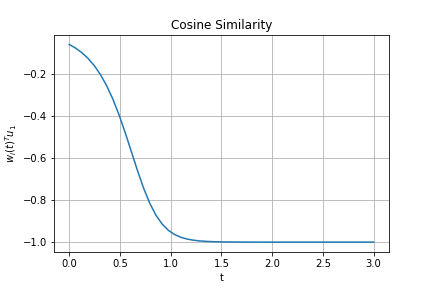
\includegraphics[width=0.45\textwidth]{Ex_02/Figures/CosSimilarity_negative.png}
    \caption{Cosine similaritity between $w(t)$ and $u_1$ for two different setups. Note that the two setups differ in the initial condition $w_0$, i.e. once $w_0^Tu_1 > 0$ (left) and once $w_0^Tu_1 < 0$ (right).}
    \label{fig:cos_sim}
\end{figure}

To get a bit more precise one can observe that the cosine similarity between the iterative approximations $w_i$ and the target $u_1$ never cross the x-axes (see figure \ref{fig:cos_sim}). What does this mean? Consider the plane containing the origin and for which $u_1$ is a normal vector. Then all the iterative approximations $w_t$ will be on the same side of the plane. This includes not just the randomly chosen initial condition $w_0$ but also the vector of convergence. Thus we see the following condition:

$$ w_t \approx sgn(w_0^Tu_1)u_1 $$

%%%%%
%%%%%
%%%%%
%%%%%
%%%%%
\color{black}




